\section{Inspiration from the Primate Visual System}
\label{sec:pvc}
\cite{kruger2013deep} argues that deep hierarchies are beneficial to computer vision systems,
and that several design principles of the primate visual system can be applied
to computer vision systems and learning of deep hierarchies.
These include hierarichal processing, separation of information channels,
feedback and balancing coded structure with learning.
Figure \ref{fig:pvc1} roughly illustrates the principles of hierarichal processing and separation of information channels
in the object recognition pathway, which includes the retina, LGN, V1 through V4, TE and TEO.
V3 is omitted from the figure, as not much is known about it.
However, information from V2 passes through V3 into V4.
Note that the strict hierarichal structure as illustrated, is not an exact representation of the primate visual system,
but rather shows some of the shortcuts between the levels of the hierarchy \citep{kruger2013deep}.
Note also that the feedback connections in the visual cortex are not visible in the figure.

\begin{figure}[h!]
\centering
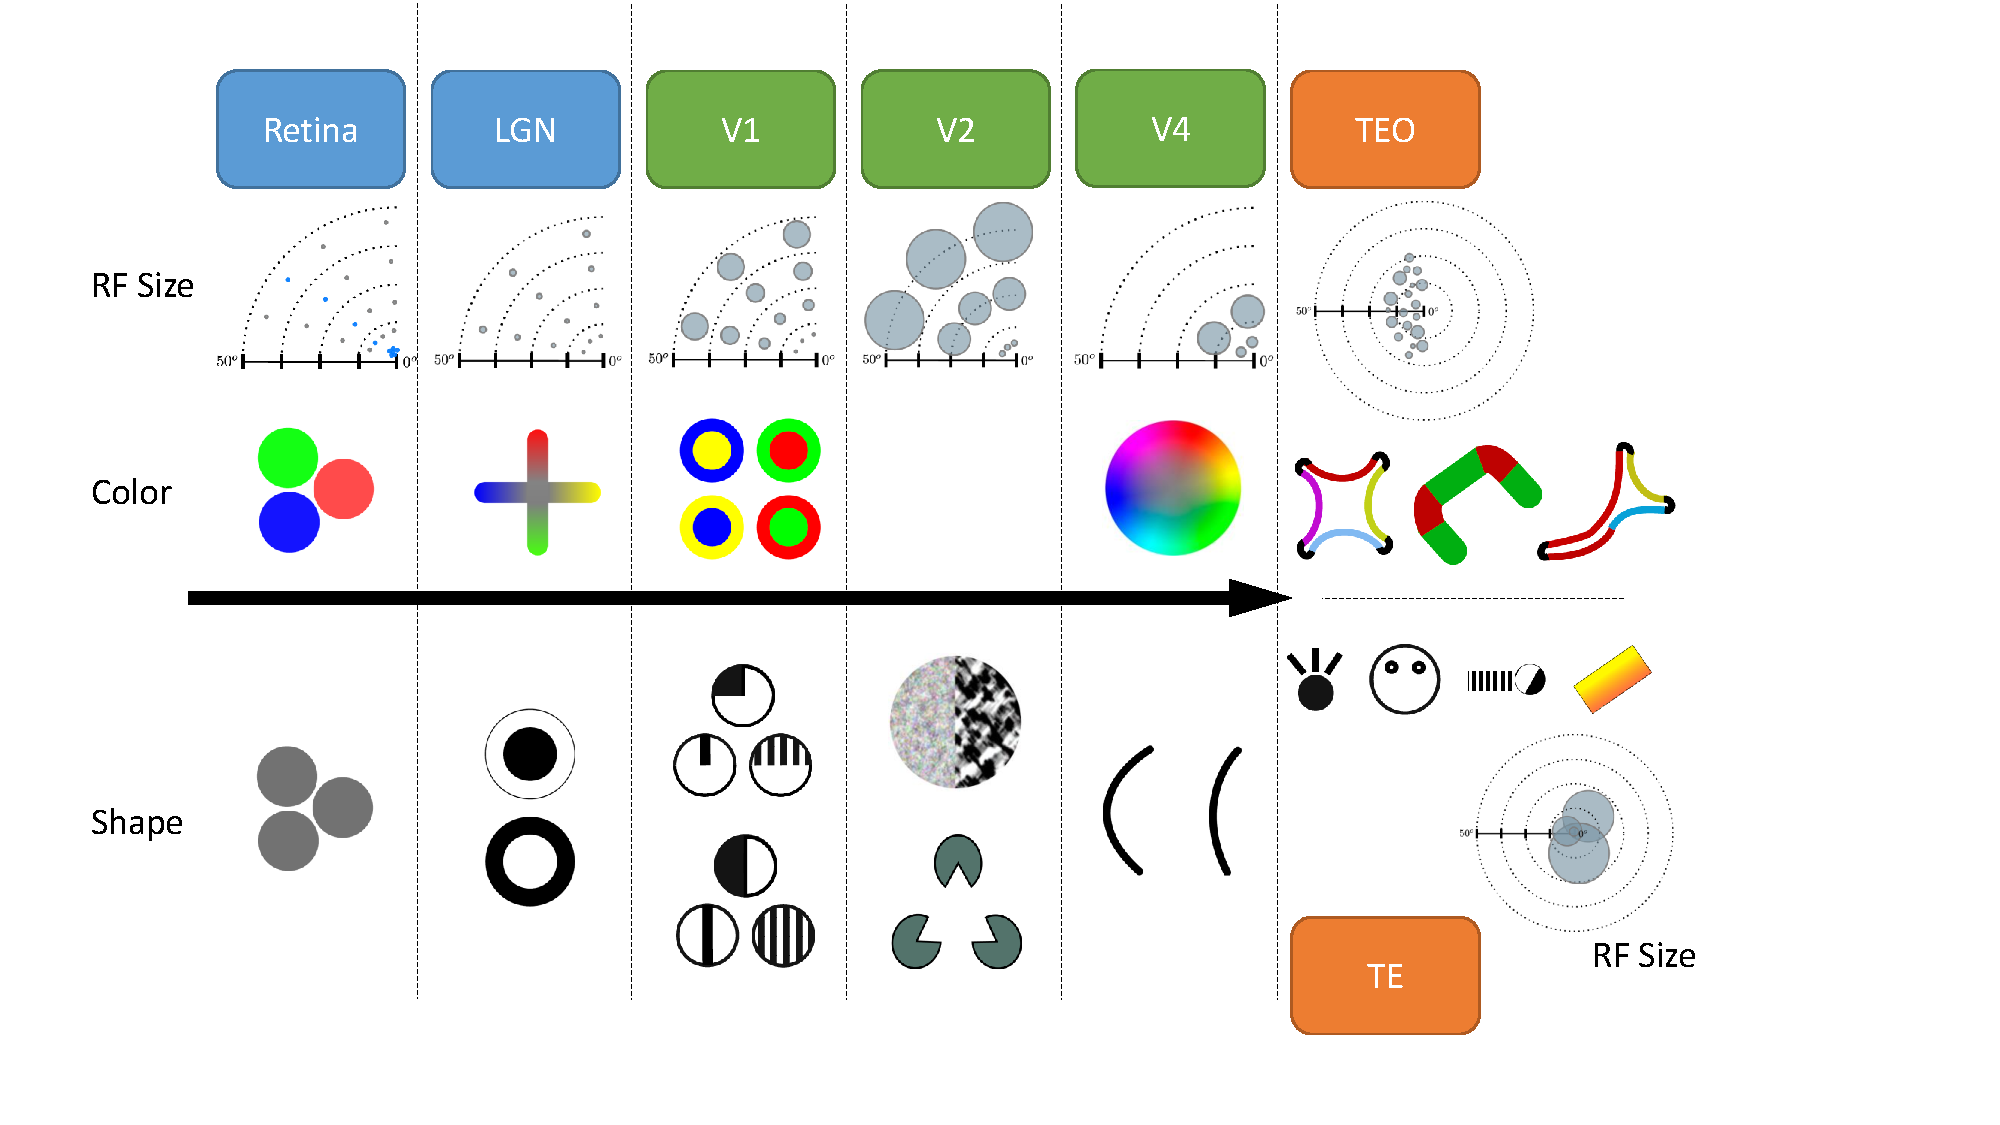
\includegraphics[width=1.1\textwidth]{graphics/pvc_figure1}
\caption[Object Recognition Pathway]{
Simplified sketch of the hierarichal structure of the object recognition pathway in the primate visual system.
The vertical lines separate layers from the low layers on the left, to the higher, more complex layers, on the right.
Up until layers TEO and TE, the compositions can be split into two categories: color and shape.
Also illustrated are the Receptive Field sizes (RF Size) of the individual layers.
Adapted from \cite{kruger2013deep}.
}
\label{fig:pcv1}
\end{figure}

Looking at figure \ref{fig:pvc1}, it is seen that the receptive field size varies throughout the layers.
This indicates a spatial distribution of the computations.
The increase in complexity of the color and space information thoughout the layers
indicates a sequential distribution of the computations as well. In summary, the object recognition pathway
is parallelized and pipelined, and, as argued in \cite{kruger2013deep},
this might be a real plus in eg. future GPUs, taking advantage of parallel computations.

The separation of information channels provides a certain robustness to the visual system:
If some visual cues are not available, for example, in the absence of color information,
the structure allows the higher layers of the visual system to trust the more reliable cues,
in this case, shape information.
Another advantage, as explained in \cite{kruger2013deep},
